\documentclass[11pt]{article}
\usepackage[utf8]{inputenc}
\usepackage{amsmath, amssymb, amsthm}
\usepackage{geometry}
\usepackage{enumitem}
\usepackage{booktabs}
\usepackage{array}
\usepackage{graphicx}
\usepackage{float}

\geometry{margin=1in}

\title{COMP 584 --- Homework 2}
\author{Dev Sanghvi \\ NetID: ds221}
\date{March 2, 2026}

\begin{document}

\maketitle

%==============================================================================
\section*{Problem 1 (25 pts): RNN Language Model}
%==============================================================================

Given
\[
\begin{aligned}
e_{t-1} &= E x_{t-1}, \\
a_t &= W_h h_{t-1} + W_e e_{t-1} + b_1, \\
h_t &= \tanh(a_t), \\
z_t &= U h_t + b_2, \\
\hat y_t &= \operatorname{softmax}(z_t),
\end{aligned}
\]
with one-hot target $y_t = x_t$, per-step loss
\[
L_t = -\sum_{j=1}^{V} y_{t,j} \log \hat y_{t,j},
\]
and total loss
\[
J = \sum_{t=1}^{T+1} L_t.
\]

%------------------------------------------------------------------------------
\subsection*{(a) Perplexity (10 pts)}
%------------------------------------------------------------------------------

By one-hot $y_t$, if the true token index at time $t$ is $k_t$, then
\[
L_t = -\log \hat y_{t,k_t} = -\log P(x_t \mid x_{0:t-1}).
\]
Hence
\[
J = -\sum_{t=1}^{T+1} \log P(x_t \mid x_{0:t-1}).
\]
Perplexity is
\[
\operatorname{PPL} = \exp\!\left(-\frac{1}{T+1}\sum_{t=1}^{T+1} \log P(x_t \mid x_{0:t-1})\right)
= \exp\!\left(\frac{J}{T+1}\right).
\]
Therefore,
\[
\boxed{\operatorname{PPL} = \exp\!\left(\frac{J}{T+1}\right)}.
\]

If the model is uniform at every step, $\hat y_{t,j} = 1/V$ for all $t,j$, then
\[
P(x_t \mid x_{0:t-1}) = \frac{1}{V},\quad
L_t = -\log\frac{1}{V} = \log V.
\]
So
\[
J = (T+1)\log V,
\quad
\operatorname{PPL} = \exp\!\left(\frac{(T+1)\log V}{T+1}\right)=\exp(\log V)=V.
\]
Thus,
\[
\boxed{\operatorname{PPL}_{\text{uniform}} = V}.
\]

%------------------------------------------------------------------------------
\subsection*{(b) Backpropagation Through Time: $\partial J/\partial W_h$ (15 pts)}
%------------------------------------------------------------------------------

Define
\[
\delta_t = \frac{\partial J}{\partial a_t} \in \mathbb{R}^H,
\]
and let
\[
g_t = \frac{\partial J}{\partial h_t}.
\]
Using the provided identity:
\[
\frac{\partial L_t}{\partial z_t} = \hat y_t - y_t.
\]
Since $z_t = U h_t + b_2$, contribution from $L_t$ to $h_t$ is
\[
\frac{\partial L_t}{\partial h_t} = U^\top(\hat y_t - y_t).
\]
Also $h_t$ affects future loss through $a_{t+1}=W_h h_t + \cdots$, giving
\[
\frac{\partial J}{\partial h_t} = U^\top(\hat y_t - y_t) + W_h^\top \delta_{t+1}.
\]
Because $h_t = \tanh(a_t)$,
\[
\delta_t
= \frac{\partial J}{\partial h_t} \odot \left(1-\tanh^2(a_t)\right)
= \left[U^\top(\hat y_t-y_t) + W_h^\top\delta_{t+1}\right] \odot (1-h_t\odot h_t).
\]
With terminal condition $\delta_{T+2}=0$, the recurrence is
\[
\boxed{
\delta_t = \left[U^\top(\hat y_t-y_t) + W_h^\top\delta_{t+1}\right] \odot (1-h_t\odot h_t),
\quad t=T+1,\dots,1.
}
\]

For $W_h$, since $a_t = W_h h_{t-1}+\cdots$,
\[
\frac{\partial a_t}{\partial W_h} = h_{t-1}^\top,
\]
so
\[
\boxed{
\frac{\partial J}{\partial W_h} = \sum_{t=1}^{T+1} \delta_t h_{t-1}^\top,
\qquad (h_0=0).
}
\]

\newpage
%==============================================================================
\section*{Problem 2 (30 pts): Understanding and Differentiating the LSTM Cell}
%==============================================================================

Let
\[
s_t = \begin{bmatrix} h_{t-1} \\ x_t \end{bmatrix} \in \mathbb{R}^{H+d}.
\]
Assume gate parameters
\[
W_f,W_i,W_o,W_g \in \mathbb{R}^{H\times(H+d)},
\quad
b_f,b_i,b_o,b_g \in \mathbb{R}^{H}.
\]

%------------------------------------------------------------------------------
\subsection*{(a) Forward Pass (10 pts)}
%------------------------------------------------------------------------------

Define pre-activations
\[
\begin{aligned}
a_t^{(f)} &= W_f s_t + b_f, \\
a_t^{(i)} &= W_i s_t + b_i, \\
a_t^{(o)} &= W_o s_t + b_o, \\
a_t^{(g)} &= W_g s_t + b_g.
\end{aligned}
\]

Gate/node activations
\[
\begin{aligned}
f_t &= \sigma\!\left(a_t^{(f)}\right), \\
i_t &= \sigma\!\left(a_t^{(i)}\right), \\
o_t &= \sigma\!\left(a_t^{(o)}\right), \\
\tilde c_t &= \tanh\!\left(a_t^{(g)}\right).
\end{aligned}
\]

Cell and hidden updates
\[
\begin{aligned}
c_t &= f_t \odot c_{t-1} + i_t \odot \tilde c_t, \\
h_t &= o_t \odot \tanh(c_t).
\end{aligned}
\]

\textbf{Operation types:}
\begin{itemize}[nosep]
    \item Affine transformations: $a_t^{(f)}, a_t^{(i)}, a_t^{(o)}, a_t^{(g)}$.
    \item Nonlinearities: $\sigma(\cdot)$ for gates, $\tanh(\cdot)$ for candidate and output squashing.
    \item Elementwise operations: $\odot$ products and vector sum in $c_t$.
\end{itemize}

\textbf{Dimensions:}
\begin{itemize}[nosep]
    \item $x_t\in\mathbb{R}^d$, $h_{t-1},c_{t-1},h_t,c_t\in\mathbb{R}^H$.
    \item $s_t\in\mathbb{R}^{H+d}$.
    \item $a_t^{(\cdot)}, f_t,i_t,o_t,\tilde c_t\in\mathbb{R}^H$.
\end{itemize}

%------------------------------------------------------------------------------
\subsection*{(b) Backward Pass: Cell-State Gradient Flow (10 pts)}
%------------------------------------------------------------------------------

Define
\[
\delta_t^h = \frac{\partial J}{\partial h_t},
\qquad
\delta_t^c = \frac{\partial J}{\partial c_t}.
\]
From
\[
h_t = o_t\odot\tanh(c_t),
\]
the local contribution is
\[
\left.\delta_t^c\right|_{\text{through }h_t}
= \delta_t^h \odot o_t \odot \left(1-\tanh^2(c_t)\right).
\]
From
\[
c_{t+1} = f_{t+1}\odot c_t + i_{t+1}\odot\tilde c_{t+1},
\]
future contribution is
\[
\left.\delta_t^c\right|_{\text{through }c_{t+1}} = \delta_{t+1}^c \odot f_{t+1}.
\]
Therefore,
\[
\boxed{
\delta_t^c
= \delta_t^h \odot o_t \odot \left(1-\tanh^2(c_t)\right)
+ \delta_{t+1}^c \odot f_{t+1}.
}
\]
This is the required recursive dependence across time (with $\delta_{T+1}^c=0$ at sequence end).

The long-term propagation term is the additive memory path multiplied by forget gates:
\[
\delta_t^c \supset \delta_T^c \odot \prod_{k=t+1}^{T} f_k,
\]
which can stay stable when $f_k\approx 1$.

%------------------------------------------------------------------------------
\subsection*{(c) Gradient w.r.t. Forget-Gate Parameters (5 pts)}
%------------------------------------------------------------------------------

For forget gate:
\[
a_t^{(f)} = W_f s_t + b_f,
\qquad
f_t = \sigma(a_t^{(f)}).
\]
Since $c_t = f_t\odot c_{t-1}+\cdots$,
\[
\frac{\partial J}{\partial f_t} = \delta_t^c \odot c_{t-1}.
\]
So
\[
\delta_t^{a_f}
:= \frac{\partial J}{\partial a_t^{(f)}}
= \left(\delta_t^c \odot c_{t-1}\right) \odot f_t\odot(1-f_t).
\]
Then
\[
\boxed{
\frac{\partial J}{\partial W_f}
= \sum_{t=1}^{T} \delta_t^{a_f} s_t^\top.
}
\]
Matrix form (stacking columns):
\[
\Delta_f = [\delta_1^{a_f},\dots,\delta_T^{a_f}]\in\mathbb{R}^{H\times T},
\quad
S=[s_1,\dots,s_T]\in\mathbb{R}^{(H+d)\times T},
\quad
\frac{\partial J}{\partial W_f}=\Delta_f S^\top.
\]

%------------------------------------------------------------------------------
\subsection*{(d) Stability Analysis (5 pts)}
%------------------------------------------------------------------------------

From
\[
c_k = f_k\odot c_{k-1}+\cdots,
\]
the Jacobian between cell states is
\[
\frac{\partial c_T}{\partial c_t}
= \prod_{k=t+1}^{T} \operatorname{diag}(f_k).
\]
If $f_k\approx 1$ for all $k$, then
\[
\boxed{\frac{\partial c_T}{\partial c_t} \approx I.}
\]

For a vanilla RNN,
\[
h_k = \phi(W_h h_{k-1}+\cdots),
\quad
\frac{\partial h_T}{\partial h_t}
= \prod_{k=t+1}^{T} D_k W_h,
\]
where $D_k=\operatorname{diag}(\phi'(\cdot))$.
This repeated matrix product often shrinks (or explodes) with time due spectral effects and saturating nonlinearities.

Hence LSTMs mitigate vanishing gradients by providing an additive memory path with near-identity Jacobian when forget gates stay near 1.

\newpage
%==============================================================================
\section*{Problem 3 (45 pts): Implementing an LSTM from Scratch}
%==============================================================================

All implementation details and executable code are provided in:
\begin{center}
\texttt{HW2.ipynb}
\end{center}

%------------------------------------------------------------------------------
\subsection*{(a) Single LSTM Cell (5 pts)}
%------------------------------------------------------------------------------

Implemented class:
\begin{center}
\texttt{LSTMCellScratch(nn.Module)}
\end{center}
with forward signature
\begin{center}
\texttt{forward(x\_t, h\_prev, c\_prev) -> (h\_t, c\_t)}.
\end{center}

Implementation properties:
\begin{itemize}[nosep]
    \item Uses affine transforms over concatenated input $[h_{t-1};x_t]$.
    \item Explicit forget, input, output, and candidate gates.
    \item Cell update and hidden update are implemented as separate elementwise operations.
\end{itemize}

%------------------------------------------------------------------------------
\subsection*{(b) Sequence Model (10 pts)}
%------------------------------------------------------------------------------

Implemented language model:
\begin{itemize}[nosep]
    \item \textbf{Embedding layer}: maps token ids to dense vectors.
    \item \textbf{Custom LSTM cell}: unrolled over sequence length.
    \item \textbf{Linear output layer}: maps each $h_t$ to vocabulary logits.
\end{itemize}

The forward pass returns logits for all time steps with shape
\[
\texttt{[batch\_size, seq\_len, vocab\_size]}.
\]

%------------------------------------------------------------------------------
\subsection*{(c) Synthetic Copy Task Results (20 pts)}
%------------------------------------------------------------------------------

Task setup: input sequence equals target sequence,
\[
(x_1,\dots,x_T) \mapsto (x_1,\dots,x_T).
\]

Training configuration used in the executed notebook:
\begin{center}
\begin{tabular}{l c}
\toprule
\textbf{Hyperparameter} & \textbf{Value} \\
\midrule
Vocabulary size & 30 \\
Embedding dimension & 32 \\
Hidden size & 64 \\
Sequence length $T$ & 30 \\
Batch size & 128 \\
Optimizer & Adam \\
Learning rate & $3\times 10^{-3}$ \\
Epochs & 20 \\
Steps per epoch & 60 \\
\bottomrule
\end{tabular}
\end{center}

Token sampling protocol: tokens are sampled uniformly over all vocabulary IDs
from $0$ to $V-1$ (no token ID is excluded).

Measured outcomes (from executed run):
\begin{itemize}[nosep]
    \item Final validation loss: $0.00029591$
    \item Final validation perplexity: $1.00029595$
    \item Final validation token accuracy: $1.0000$
    \item Cell-state gradient norm range: $\min=6.31\times 10^{-8}$, $\max=6.867\times 10^{-7}$
\end{itemize}

\begin{figure}[H]
    \centering
    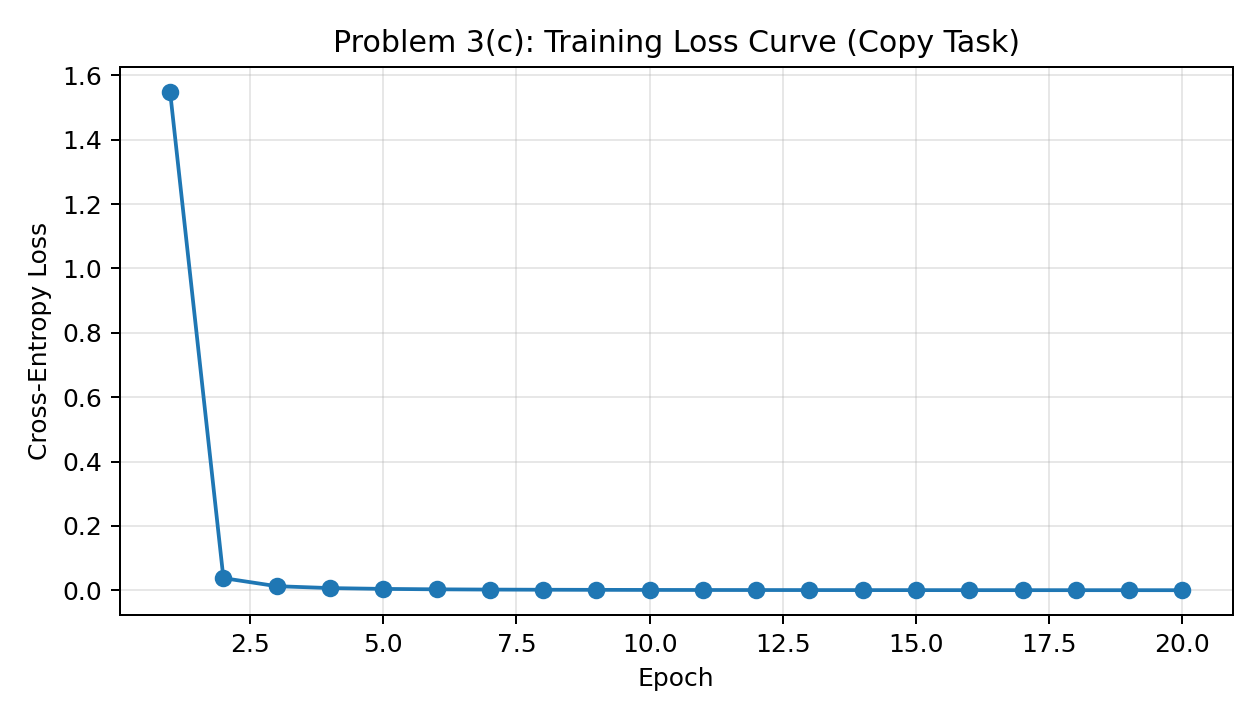
\includegraphics[width=0.78\textwidth]{figures/problem3_loss_curve.png}
    \caption{Training loss curve for the scratch LSTM on the copy task.}
\end{figure}

\begin{figure}[H]
    \centering
    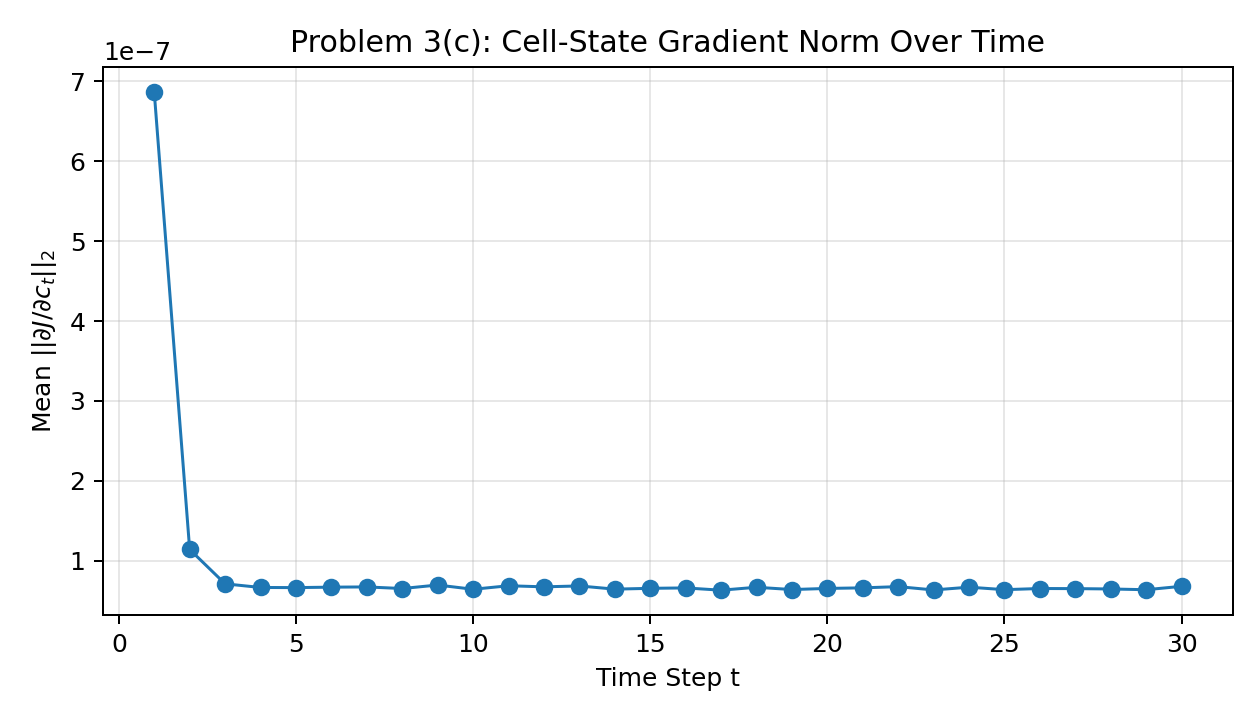
\includegraphics[width=0.78\textwidth]{figures/problem3_cell_grad_norm.png}
    \caption{Cell-state gradient norm over time steps.}
\end{figure}

%------------------------------------------------------------------------------
\subsection*{(d) Q\&A (10 pts)}
%------------------------------------------------------------------------------

Vanilla RNNs face several structural limitations in NLP. First, sequence processing is strictly recurrent, so computation is sequential across time and cannot be fully parallelized during training; this limits throughput on long texts. Second, gradients pass through many repeated Jacobian multiplications, which makes optimization unstable due vanishing or exploding gradients, especially for long contexts. Third, hidden-state compression into a fixed-size vector bottleneck can lose fine-grained token interactions and long-range dependencies. Fourth, recurrence has a long effective path length between distant tokens, so learning dependencies across far-apart words is difficult.

Transformers address these issues with self-attention. Every token can directly attend to every other token in the same layer, so long-distance interactions have short gradient paths. Attention and feed-forward blocks are highly parallelizable across token positions, greatly improving hardware utilization and training speed. Multi-head attention captures multiple relation types simultaneously, and deep stacks with residual connections plus normalization improve optimization stability. With positional encodings and scaling, Transformers model both local and global context effectively, which is why they outperform RNNs on modern NLP tasks.

\vspace{1.5em}
\hrule
\vspace{0.8em}

\noindent\textbf{Submission files prepared:}
\begin{itemize}[nosep]
    \item \texttt{HW2.pdf} (this report)
    \item \texttt{HW2.ipynb} (full coding implementation and outputs)
    \item \texttt{NLP\_HW2\_ds221.zip} (submission bundle)
\end{itemize}

\end{document}
